% Compiler ce document 

% package de base
\documentclass[10pt,a4paper]{article}
\usepackage[utf8]{inputenc}
\usepackage{listings}

% langues
\usepackage[usenames,dvipsnames]{xcolor}
\usepackage[francais]{babel}
\usepackage[T1]{fontenc}
\usepackage{amsmath}
\usepackage{amsfonts}
\usepackage{amssymb}
\usepackage{graphicx}
\usepackage{tabularx}
\usepackage{colortbl}
\usepackage[hidelinks]{hyperref} % liens
\usepackage{fancyhdr} % En tetes / bas de page
\usepackage{helvet} % police helvetica
\usepackage[hidelinks]{hyperref}
\usepackage{xcolor} % Style pour affichage du C
\usepackage{courier} % police pour les listings
\usepackage{tikz}

\usepackage{listingsutf8}

% Page de Garde -- Necessite d'installer le package titling, si probleme
% commenter la ligne suivante ainsi que les infos necessaires a la page
% de garde
\usepackage{pageGarde/Garde_perso}

% commande pour faire des sections sans nombre 
% tout en la rajoutant dans la table des matières
\newcommand\sectionWithoutNumber[1]{\section*{#1} \addcontentsline{toc}{section}{\protect\numberline{}#1}}
\newcommand\subsectionWithoutNumber[1]{\subsection*{#1} \addcontentsline{toc}{subsection}{\protect\numberline{}#1}}
\newcommand\subsubsectionWithoutNumber[1]{\subsection*{#1} \addcontentsline{toc}{subsubsection}{\protect\numberline{}#1}}
% définition de nouvelles couleurs
\definecolor{lightblue}{rgb}{0.8,0.8,0.9}
\definecolor{grossblue}{rgb}{0,0,0.7}
%marge des pages
\setlength{\textwidth}{16cm}
\setlength{\textheight}{24cm}
\setlength{\oddsidemargin}{0cm}
\setlength{\voffset}{-1.5cm}
\setlength{\headheight}{15pt}

% set la police en arial
%% Sans-serif Arial-like fonts
\renewcommand{\rmdefault}{phv} 
\renewcommand{\sfdefault}{phv} 
\usepackage{tabularx}
\usepackage{graphicx}
\usepackage{eurosym}
\usepackage{xspace}
\newcommand{\projectname}[0]{LTANR\xspace} 

% configuration pour des listings
\lstset{ 
  showspaces=false,      
  showstringspaces=false, 
  showtabs=false,               
  tabsize=3,                     
  numbers=left
}

%enlève indentation en début de paragraphe
\setlength\parindent{0pt}

%style de l'en-tête de page
\pagestyle{fancy}

% style pour code en c
\lstdefinestyle{customc}{
  belowcaptionskip=1\baselineskip,
  breaklines=true,
  frame=L,
  xleftmargin=\parindent,
  language=C,
  showstringspaces=false,
  basicstyle=\scriptsize\ttfamily,
  keywordstyle=\bfseries\color{green!40!black},
  commentstyle=\itshape\color{purple!40!black},
  identifierstyle=\color{blue},
  stringstyle=\color{orange},
}

\lstdefinelanguage{VHDL}{
      morekeywords=[1]{
        library,use,all,entity,is,port,in,out,end,architecture,of,
        begin,and,or,Not,downto,ALL
      },
      morekeywords=[2]{
        STD_LOGIC_VECTOR,STD_LOGIC,IEEE,STD_LOGIC_1164,
        NUMERIC_STD,STD_LOGIC_ARITH,STD_LOGIC_UNSIGNED,std_logic_vector,
        std_logic
      },
      morecomment=[l]--
    }
    \usepackage[usenames,dvipsnames]{xcolor}
    \colorlet{keyword}{blue!100!black!80}
    \colorlet{STD}{Lavender}
    \colorlet{comment}{green!80!black!90}
    \lstdefinestyle{vhdl}{
      language     = VHDL,
      basicstyle   = \footnotesize \ttfamily,
      keywordstyle = [1]\color{keyword}\bfseries,
      keywordstyle = [2]\color{STD}\bfseries,
      commentstyle = \color{comment}
      breaklines=true,                % sets automatic line breaking
      tabsize=3                                % sets default tabsize to 2 spaces
    }

\lstset{escapechar=@,style=customc}
\lstset{inputencoding=utf8/latin1} %affiche les accents dans le listing

% Mise en forme de la page de titre
\author{João Miguel Domingues Pedrosa\\Rick Wertenbroek}
\title{Mémoire cache}
\dest{}

% Informations necessaires a la page de garde
% Commenter si probleme de compilation
\acro{CSF}
\matter{Conception de système numérique sur FPGA}
\date{\today}

%en-tête
\lhead{Domingues \& Wertenbroek}
\chead{Mémoire cache}
\rhead{\theAcro}

%pied-de-page
\lfoot{HEIG-VD}
\cfoot{\today}
\rfoot{\thepage}

\begin{document}
\maketitle
\newpage
\tableofcontents
\newpage

%Ici commence réelement l'écriture du rapport
\section{Introduction}
Lors de ce laboratoire nous avons implémenté une mémoire cache. Mémoire qui sera directement implantée dans un design FPGA. Le but d'une mémoire cache étant de diminuer le temps des lectures et écritures en évitant de devoir accéder la mémoire à chaque fois. Notre implémentation de mémoire cache sera utilisée par un (et un seul) agent et interfacera une mémoire (par exemple RAM DDR, qui sera dans ce laboratoire simulée en VHDL).

\section{Mémoire Cache}
\subsection{Mémoire}
Pour ce laboiratoire nous avons implémenté la mémoire cache comme une cache à correspondance directe avec des lignes de 16 mots, ceci s'adapte en fonction des paramètres génériques (si l'adresse devient plus longue et la taille du tag et de l'index ne changent pas les lignes auront plus de mots. Nous avons aussi testé avec des tag et index plus grands qui nous donnaient des lignes de cache de 2 mots, cela fonctionnait aussi, mais c'était bien sur moins performant...).

La mémoire se sépare en plusieurs lignes qui ont les attributs suivants :\\

\begin{itemize}
	\item Data (vecteur): il s'agit des donnée (dans le tests bench 16 mots par ligne).
	\item Tag  (vecteur): la mémoire cache est plus petite que la RAM il y a alors collisions, le tag permet de savoir si l'adresse correspond à la ligne.
	\item Valid (bit): indique si la ligne en cache est initialisée. (Si les données proviennent de la mémoire, car au reset les registres ne sont pas initialisés et la cache peut contenir n'importe quoi.
	\item Dirty (bit): indique si il y a eu un accès en écriture dans la ligne. Ces lignes devront d'abord être écrites en mémoire avant de les remplacer.\\
\end{itemize}

Pour chaque attribut, nous avons un tableau de la taille du nombre de lignes de la cache que l'on accédera grâce à l'index bits après le tag dans l'adresse recherchée par l'agent.

\newpage

\subsection{Contrôleur}
Pour le contrôleur de la mémoire cache nous avons créé une machine séquentielle synchrone.

\begin{center}

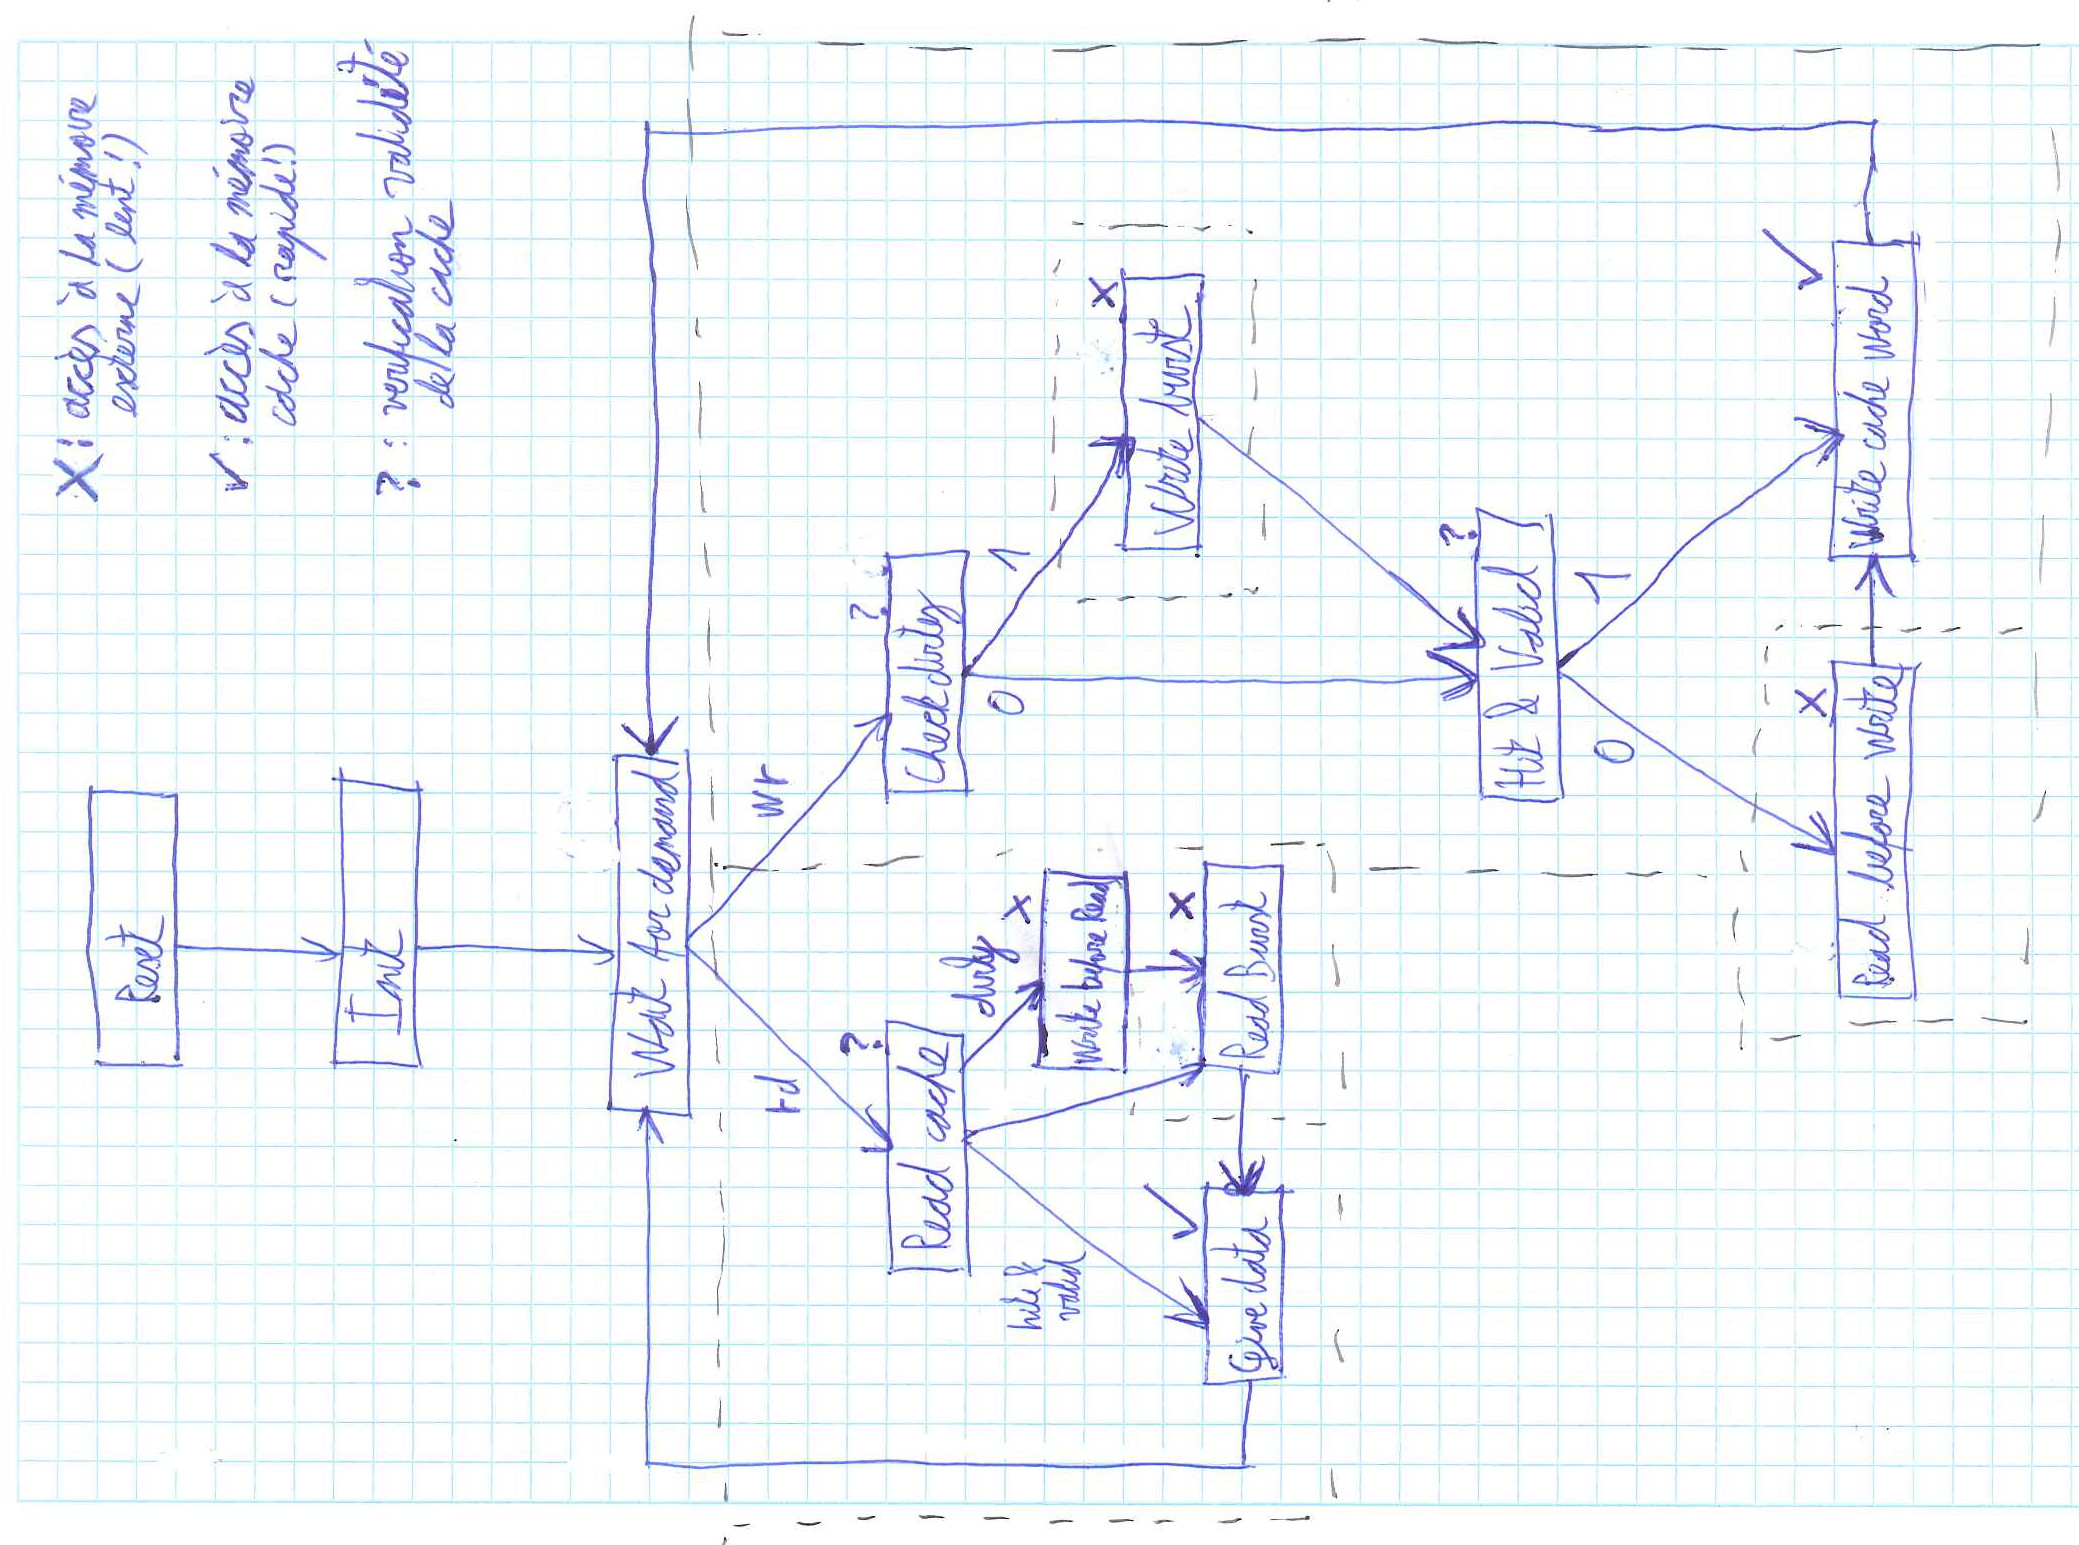
\includegraphics[width=1.3\textwidth, angle=-90]{images/mss}

\end{center}

\newpage

On commence tout d'abord par une initialisation des différents attributs de la cache. Il s'agit notamment de mettre les bits \texttt{valid} et \texttt{dirty} à 0 pour indiquer que la cache est vide (non initialisée en fait) et qu'elle doit donc être remplie avant lecture (son contenu peut être aléatoire).\\

Ensuite, dans \texttt{wait for demand}, on attend un signal (une demande) de lecture ou écriture (\texttt{rd} ou \texttt{wr}). On active le signal \texttt{busy} pour indiquer qu'on est occupé et on redirige dans la partie concernée. Il sera désactivé une fois l'action terminée.

\subsubsection{Lecture}
Pour la lecture, on vérifie d'abord s'il y a un hit. Pour cela, on regarde si le tag trouvé via l'adresse correspond à celui en cache et que la ligne est valide.
Si la réponse est positive, on récupère directement la valeur dans la mémoire cache, sinon on doit chercher la ligne en mémoire d'abord. Avant de mettre à jour la ligne de la cache, on vérifie que la ligne actuelle n'est pas \texttt{dirty} si le tag est différent. Dans ce cas il faut d'abord l'écrire en mémoire avant de la remplacer par une nouvelle.
L'accès en mémoire se fait à chaque fois en burst (plus rapide et plus simple) de la manière suivante:

\begin{center}

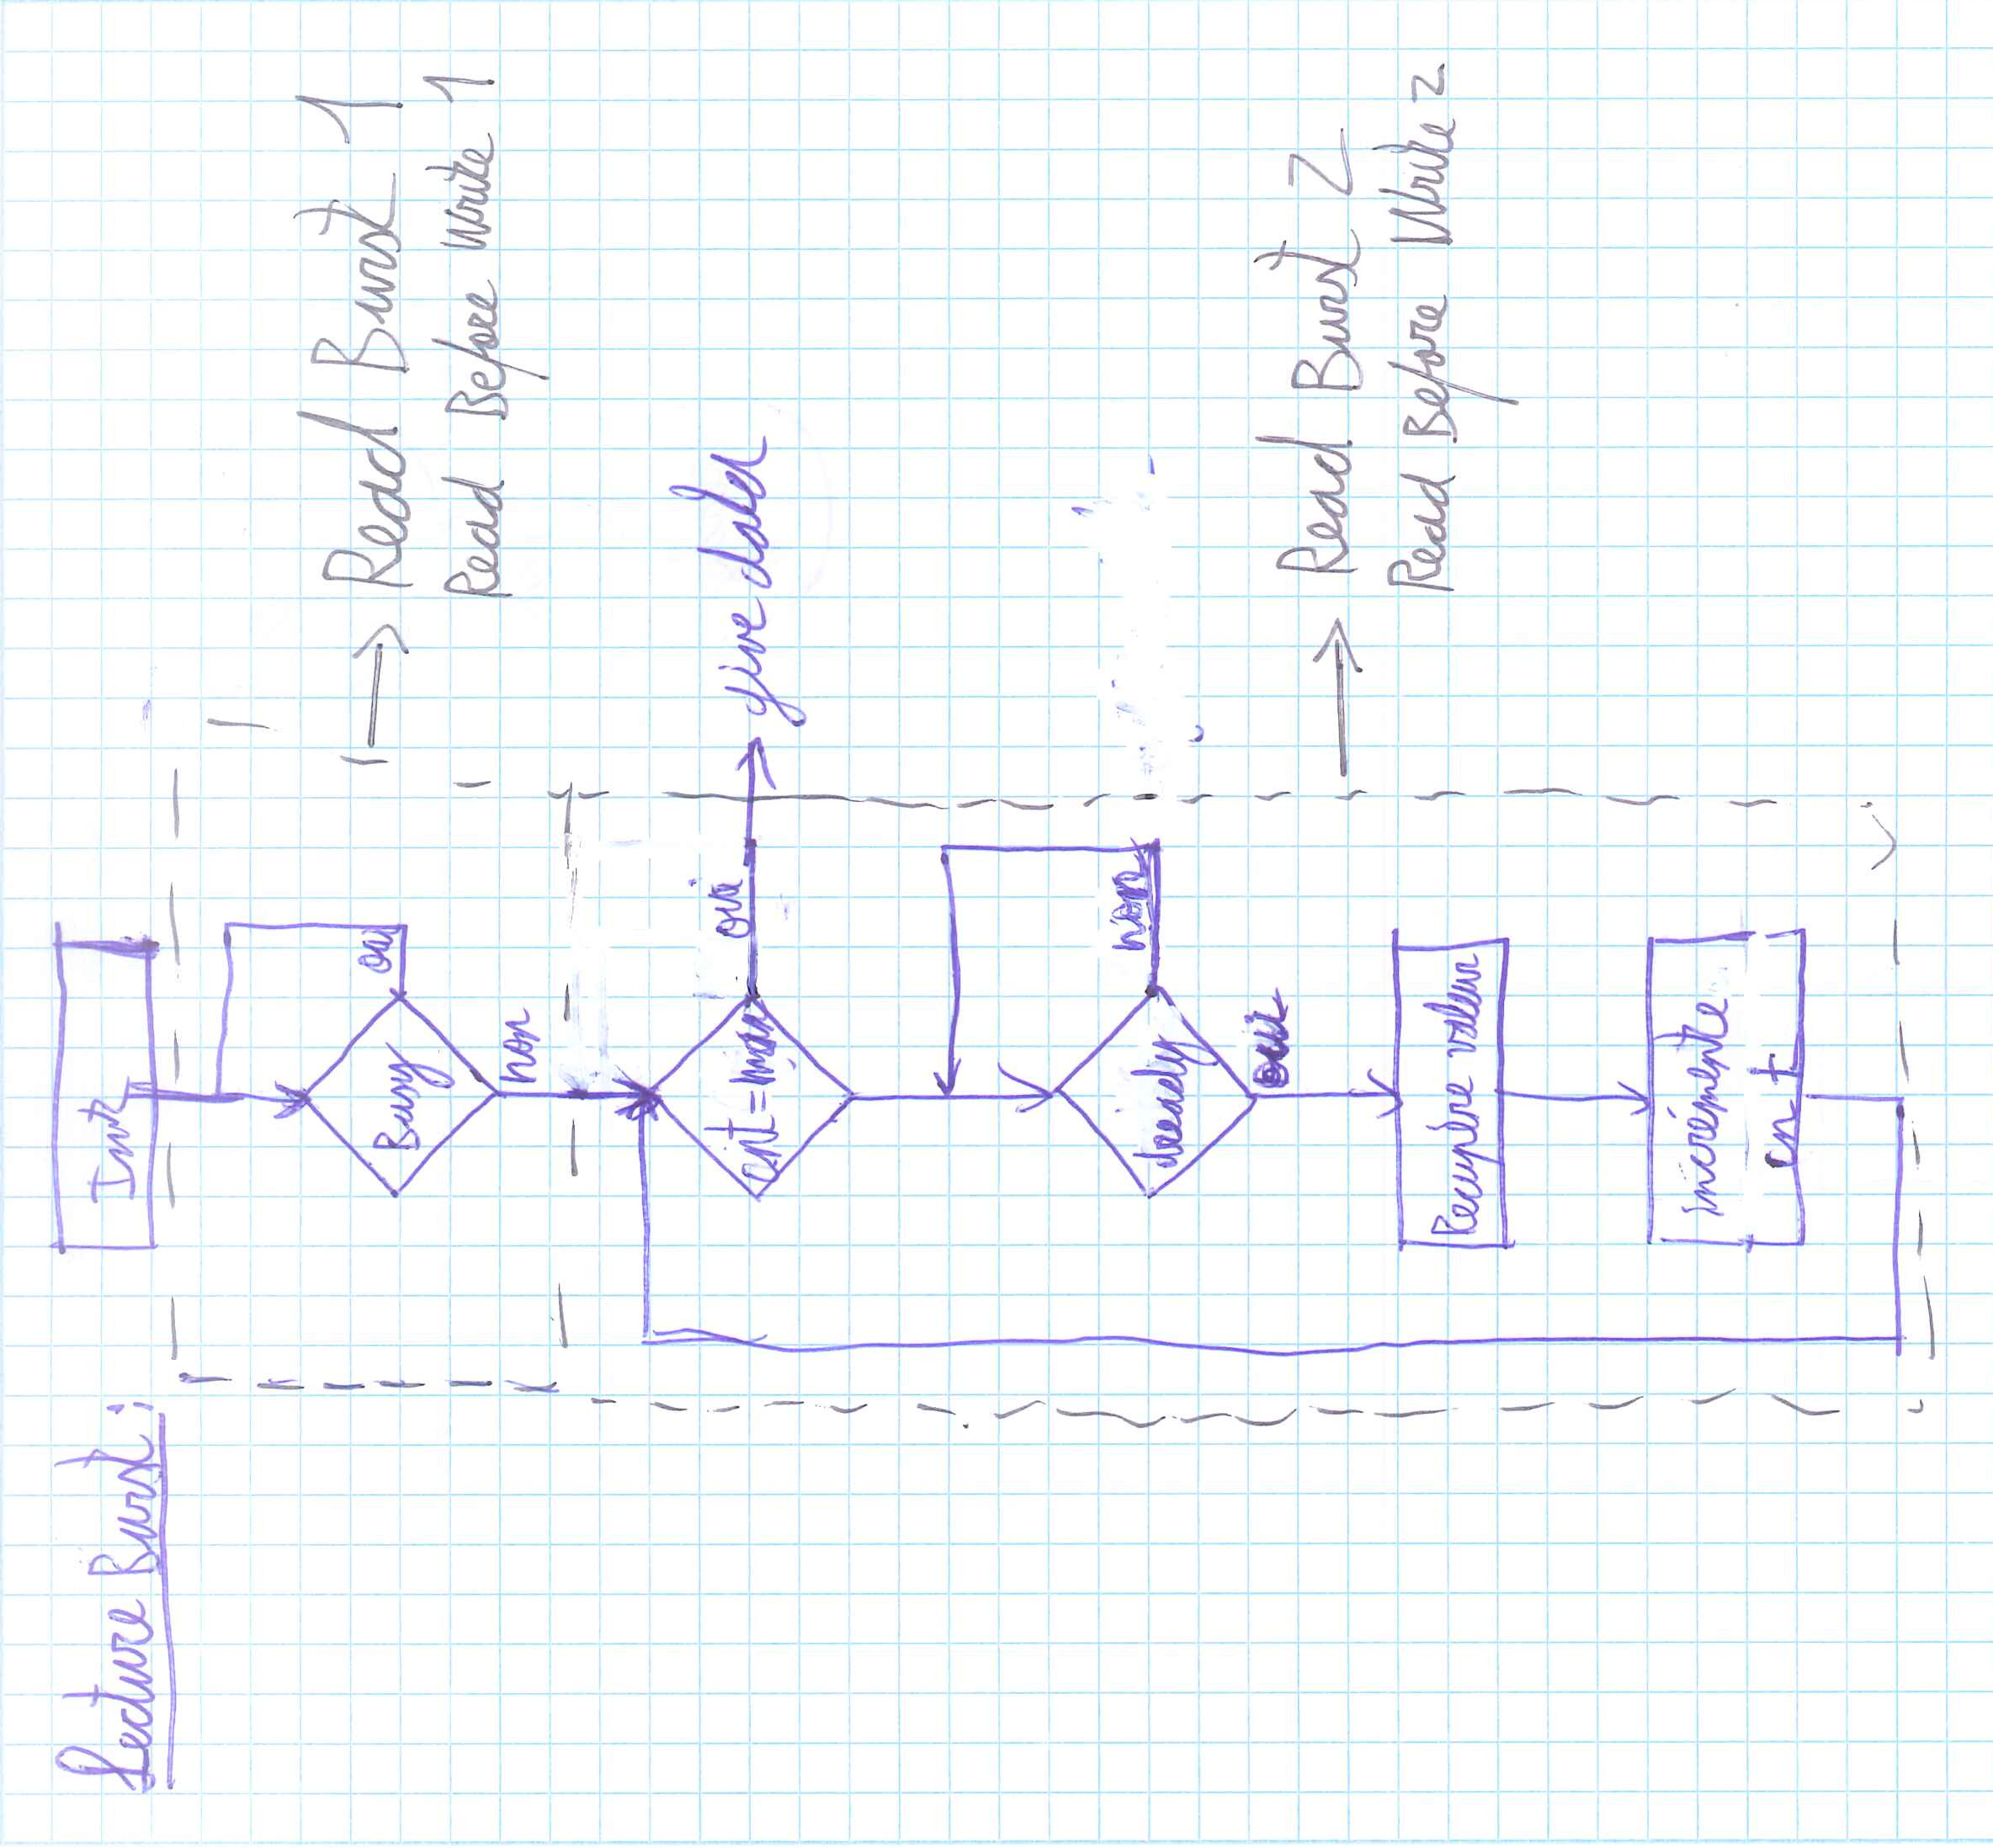
\includegraphics[width=0.7\textwidth, angle=-90]{images/mss_read}

\end{center}

On attend tout d'abord sur le busy car il se peut que la mémoire soit occupé lorsqu'on veut l’accéder. Une fois la mémoire libre, on lui demande les données, on vérifie qu'elles soient prêtes via le \texttt{dready} et les enregistres. On regarde que la mémoire à finit le transfère via un compteur que l'on incrémente à chaque fois qu'une donnée a été récupéré avec succès.

\subsubsection{Écriture}
Lors de l'écriture il y a plusieurs choses à vérifier. Si il y a déjà une ligne de cache valide appartenant à une autre adresse et qu'elle a été modifiée (dirty) il faudra la stocker en mémoire avant de la remplacer. Ensuite il faudra récupérer en mémoire la ligne sur laquelle on veut écrire afin qu'elle soit cohérente (Read before write). Une fois que la ligne a été cherchée en mémoire elle est bien-sur valide et une fois qu'on y a écrit notre valeur on lui met à jour le bit dirty.

L'écriture se fait en burst et se fait de la manière suivante:  
\begin{center}

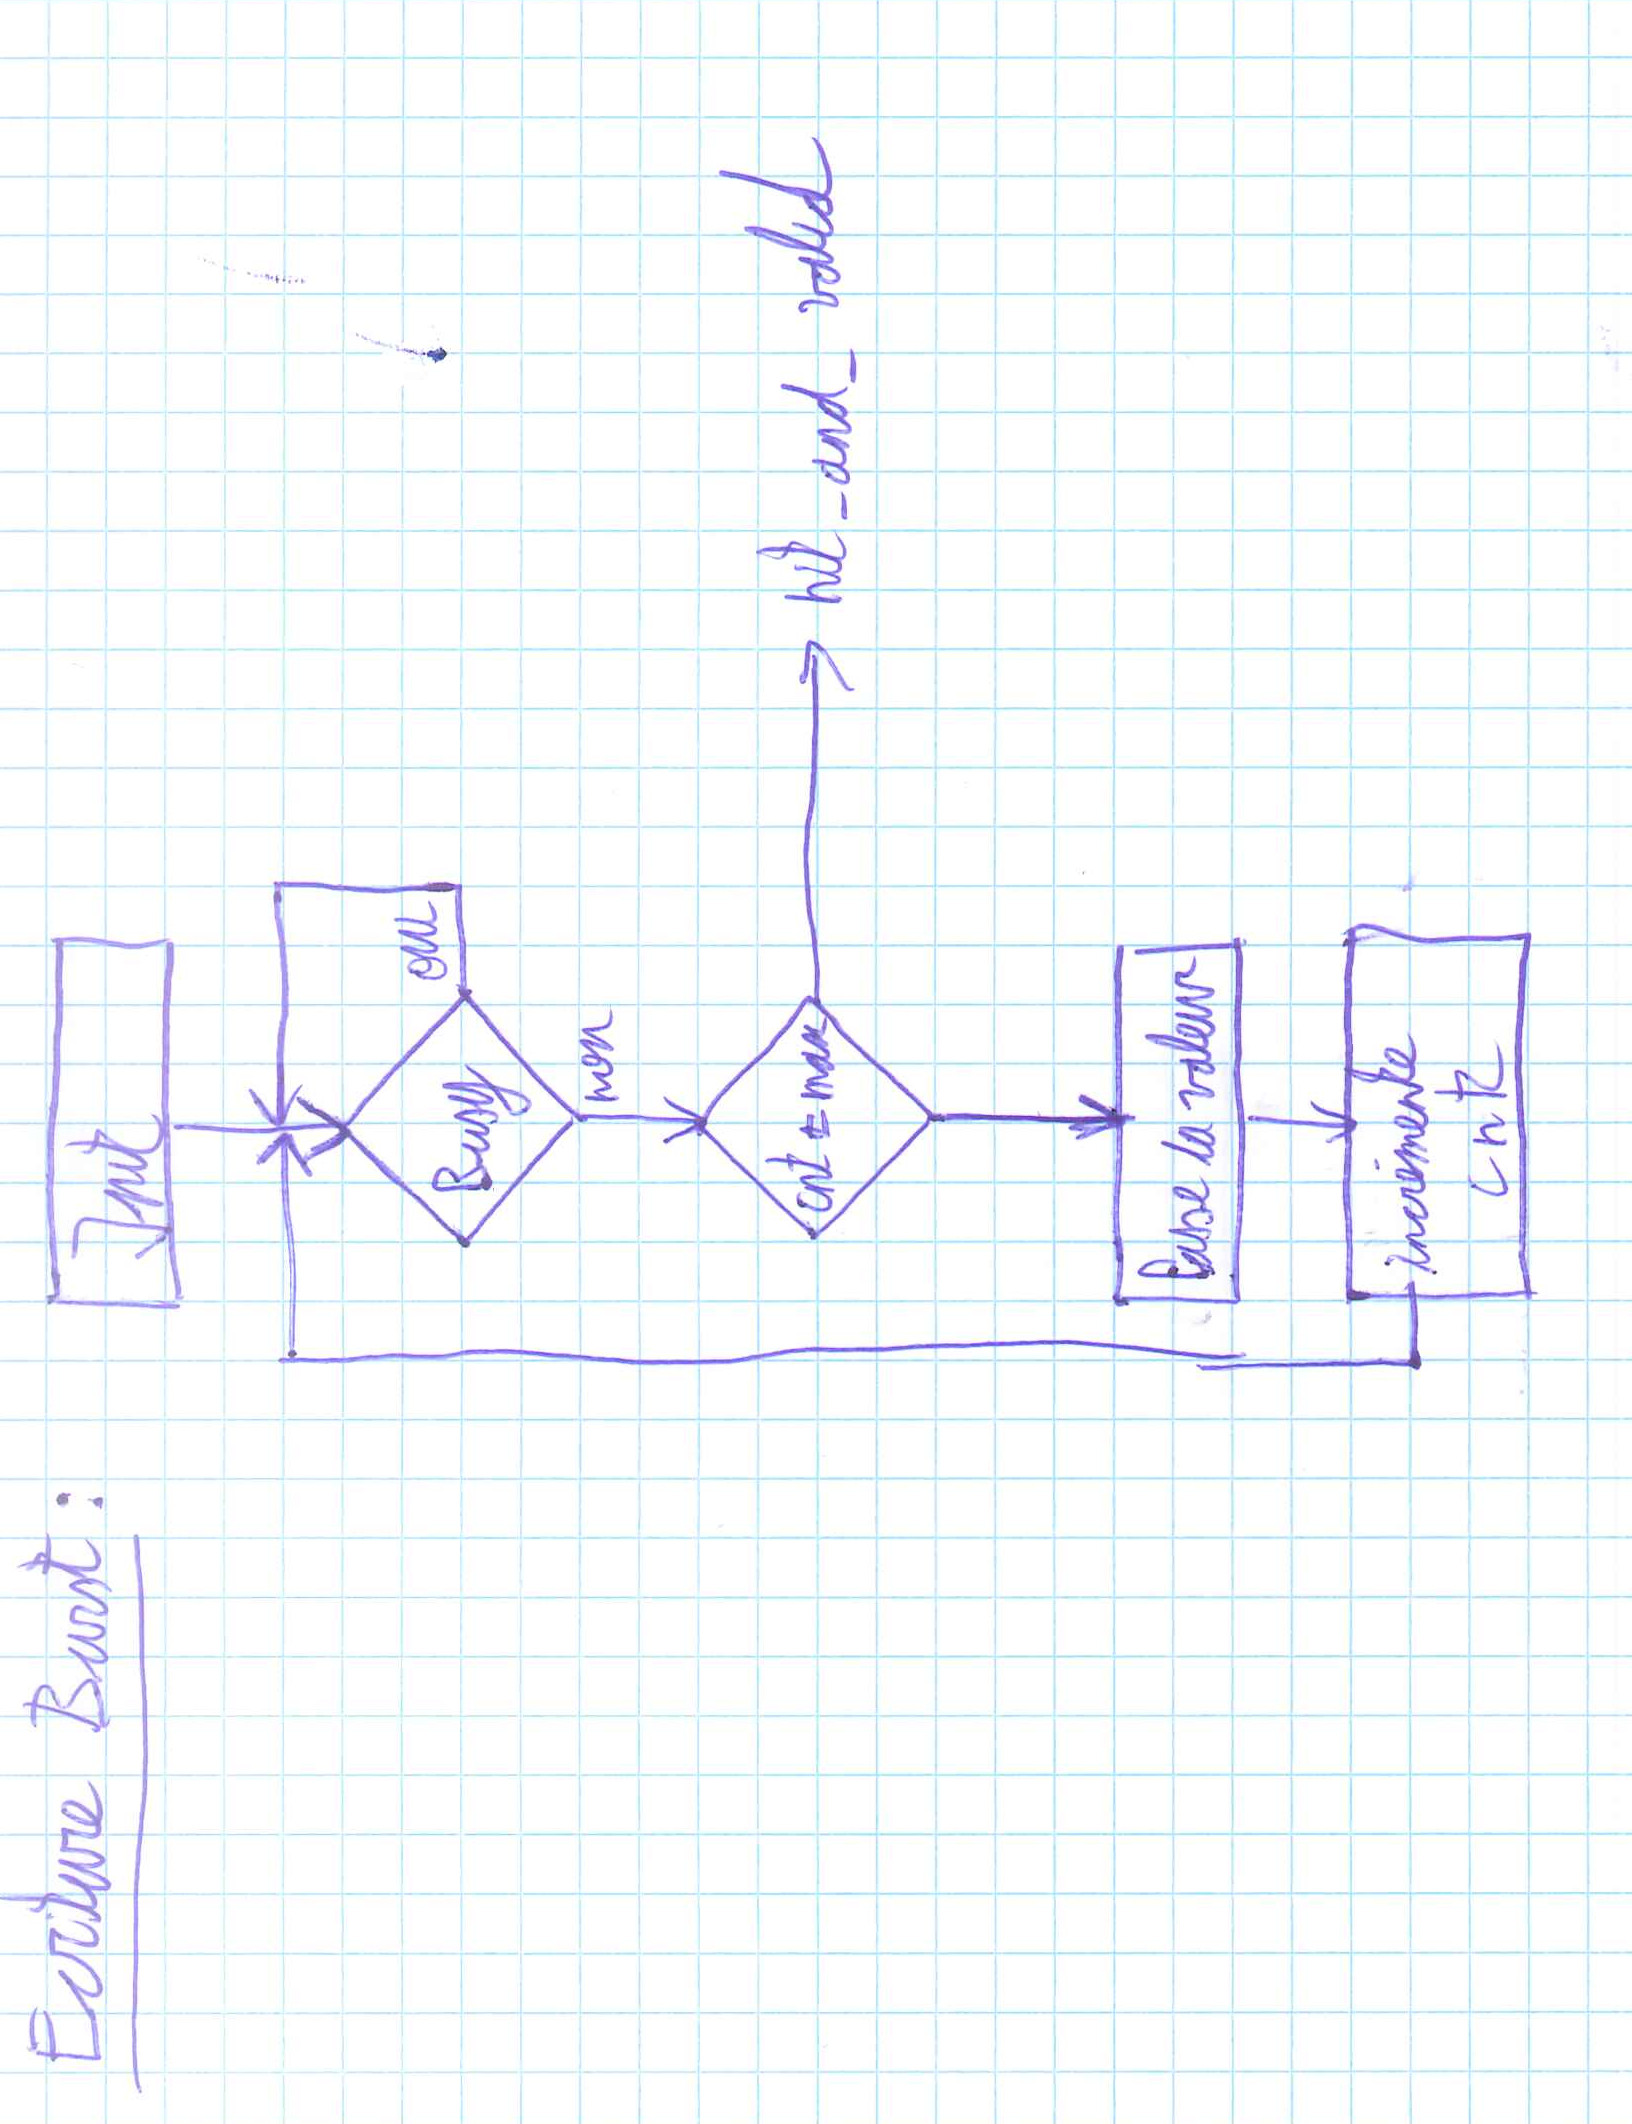
\includegraphics[width=0.5\textwidth, angle=-90]{images/mss_write}

\end{center}
Par rapport à la lecture (Read before Write), on n'attend toujours sur le signal \texttt{dready} de la mémoire.\\

En résumé, pour l'écriture on a quatre cas :
\begin{enumerate}
\item La ligne de cache est vide : il faut aller chercher la ligne dans la mémoire (et donc mettre à jour le tag et le bit valid) puis on la modifie et met le bit dirty.
\item La ligne de cache correspond à l'adresse à écrire : il suffit de modifier la ligne et mettre le bit dirty.
\item La ligne de cache contient un autre tag non dirty : on traite comme le premier cas.
\item La ligne de cache contient un autre tag et est modifiée (dirty) : on doit stocker ces informations en mémoire puis on traite comme le premier cas.
\end{enumerate}

\section{Mémoire simulée}
Pour la mémoire simulée nous avons créé une petite mémoire de 256*8bits qui peut être accédée de manière directe ou en burst, elle utilise des signaux busy et dready pour communiquer son état. La latence est simulée en attendant un nombre de coups de clocks qui est défini dans une constante. La latence aurait aussi pu être simulée ainsi : wait for xxx ns; wait until rising\_edge(clk\_i); afin de pouvoir spécifier des latences en terme de temps minimaux (xxx ns) et rester quand même synchrone.

Le fichier correspondant est memory\_emul\_tb.vhd 
\section{Banc Test}
Pour notre banc test nous avons vérifié le bon fonctionnement de la mémoire cache pour :\\
\begin{itemize}
\item Des cas de bord :
Écrire après une écriture, on devrait voir que la seconde écriture se fait bien plus vite car on n'a pas besoin d'aller chercher la ligne en mémoire. On voit bien dans le chronogramme que le premier accès prends plus de temps (lecture burst de la ligne).\\
Écrire dans une adresse puis dans la suivante qui est dans la même ligne, on voit ici que la deuxième lecture est plus rapide, pour les mêmes raisons que ci-dessus.
Lire la mémoire à une adresse pas encore en cache puis l'adresse suivante, on voit que la première lecture est lente puis la deuxième très rapide car la ligne est déjà cachée.\\
Écrire à deux adresses qui donnent le même index dans la cache (on a donc une collision) et voir que les données qui étaient présentes dans la cache se trouvent bien stockées en mémoire avant que la cache soit mise à jour.\\

\item Un parcours ascendant de toutes les adresses de la mémoire simulée :
On parcourt ici toute la plage d'adresse en écriture puis en lecture, on va voir que la cache sera mis à jour en conséquence et qu'on ne perds aucune information, tout est stocké dans la cache ou la mémoire le cas échéant. Après qu'une ligne a du être mise à jour dans la cache tous les accès suivants à cette même ligne sont rapides. Ce test provoque aussi des collisions, faire toutes les écritures puis tout relire nous permet de nous assurer qu'aucune donnée n'a été perdue (car il y a forcément des flush de la cache vers la mémoire à cause des collisions).\\

\item Un parcours descendant de toutes les adresses de la mémoire simulée :
Même idée que le test ci-dessus mais cette fois ci on devra chercher les lignes en mémoire depuis l'adresse de poids fort et on peut voir que cela fonctionne tout aussi bien. Les accès aux adresses en dessous sont donc plus rapides, jusqu'à ce que l'on doive recharger une nouvelle ligne de la mémoire vers la cache. On voit aussi que toutes les données sont préservées.\\

\item Des accès locaux successifs :
On essaie de simuler ici un usage un peu normal de la cache, plusieurs écritures successives à des lignes proches les unes des autres, puis après toutes ces écritures on observe que les données sont bien correctes. On peut voir qu'une fois la ligne chargée en cache (16 mots et on accède 10 mots) qu'on ne travaille que dans la cache et qu'il n'y a pas d'accès à la mémoire ici. Tout est très rapide et on peut le voir dans le chronogramme.\\
\end{itemize}

La procédure control\_read nous permet de vérifier la cohérence des données pour une adresse donnée en cache, il y aura une failure dans le cas contraire. (il aurait été bien de faire une collection des erreurs et indiquer à la fin du test bench le nombre d'erreurs et les adresses) mais pour l'instant nous avons simplement fait générer une failure.

\section{Synthèse}
Notre implémentation est synthétisable, la synthèse a été effectuée avec Quartus II. Il faut toutefois faire attention à définir les tailles des vecteurs dans les records du package cmf\_pkg.vhd sans cela la synthèse ne passera pas.

\section{Conclusion}
Implémenter une mémoire cache n'était pas si simple que ça, il a fallu beaucoup penser au cas de bord comme les collisions par exemple afin de ne pas faire d'erreurs. Ce n'est pas évident de prévoir qu'une lecture demandera de stocker des informations en mémoire par exemple... Une fois tous les cas de bord étudiés, la machine d'état élaborée en conséquence, le test bench a pu nous faire découvrir les failles restantes dans notre design. Avec les latences choisies (env 10 cycles d'horloge par data de la ram) il est impressionnant de voir la différence de temps entre un cache miss et un hit. Lorsque le contrôleur doit aller chercher la ligne en mémoire il lui fait plus de 160 cycles (16 mots * 10cycles plus tous les cycles de contrôle) donc environ 200 cycles, et après une fois que la ligne est chargée, tous les accès (en lecture comme en écriture) se font en quelques cycles (<10). Sur le chronogramme on voit réellement la différence. Les attentes sur la mémoire sont bien lent ! D'où l'avantage énorme d'avoir une mémoire cache.

Ce laboratoire nous a permis de mieux comprendre le fonctionnement (et surtout l'implémentation) d'une mémoire cache et de bien se rendre compte encore une fois à quel point elle est utile et le gain énorme de temps qu'elle fournit. Le test bench nous donne confiance en notre design et je suis sur que si le laboratoire avait été à rendre sans faire de banc test que notre mémoire cache aurait bien des soucis dans de nombreux cas.

\end{document}